\documentclass[10pt,a4paper]{article}
\usepackage[margin=17mm]{geometry}
\usepackage[T1]{fontenc}
\usepackage{lmodern,amsmath,amssymb,graphicx,booktabs,array,xcolor,hyperref}
\hypersetup{colorlinks=true,urlcolor=blue,pdftitle={Genuine genus-two torsion and prime-field elliptic--Richelot chains}}
\setlength{\parindent}{0pt}\setlength{\parskip}{5pt}\setcounter{secnumdepth}{0}
\newcolumntype{L}[1]{>{\raggedright\arraybackslash}p{#1}}
\newcommand{\uv}{\texttt{[pcc:unverified]}}
\begin{document}
{\LARGE\bfseries Genuine genus-two transfers}\par
{\large Actual torsion, prime-field codomains and elliptic--Richelot chains}\par
23 November 2026 \quad Chained ECDLP Transfers \quad PR 5007 / queue 3904

\fcolorbox{blue!40!black}{blue!4}{\parbox{0.95\linewidth}{
\textbf{Observed component.} An explicit elliptic pullback and two actual
Richelot chains each map all seven points of the same $E(\mathbb F_3)$ to
seven distinct valid, Frobenius-fixed Jacobian classes. Every one of the
$49$ addition pairs per map passes; total $147$. These are unsigned native
qualification records, not signed PCC or Lean verdicts. \uv}}

\section{The maps actually evaluated}
The source is $E/\mathbb F_3:Y^2=X^3+2X+1$, with its entire order-$7$
group. The intermediate curve is $C:y^2=x^6+x^5+x^2+1$. The two smooth
codomains keep their exact leading coefficients, including the nonsquare
coefficient $2$ on the second sextic. Each Richelot kernel has order $4$;
the elliptic pullback comes from a degree-$2$ cover. \uv

\begin{center}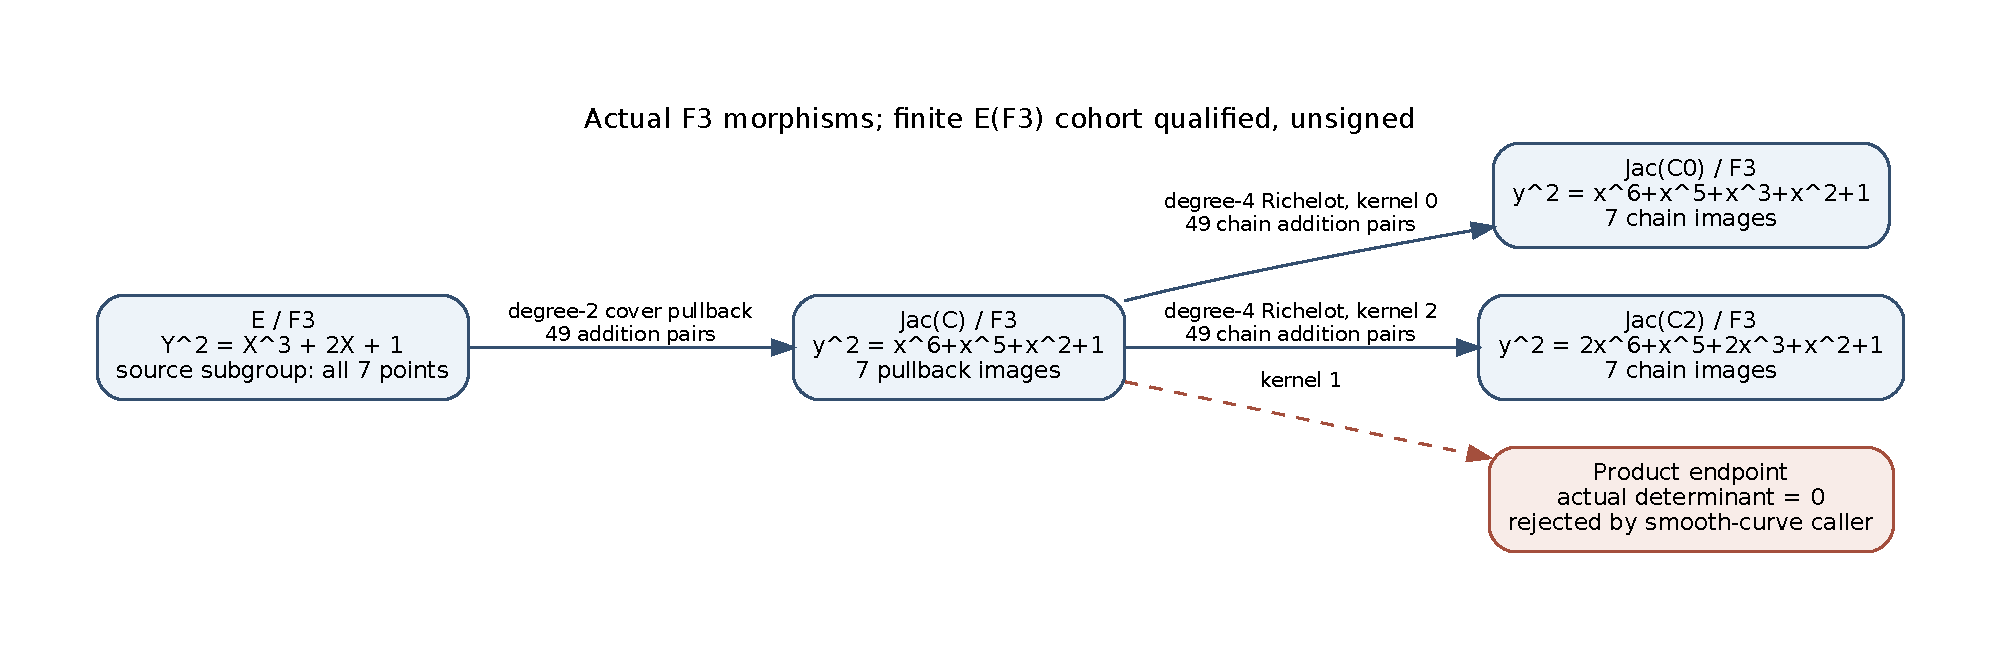
\includegraphics[width=\linewidth]{chain.pdf}\end{center}
\vspace{-2mm}
\begin{center}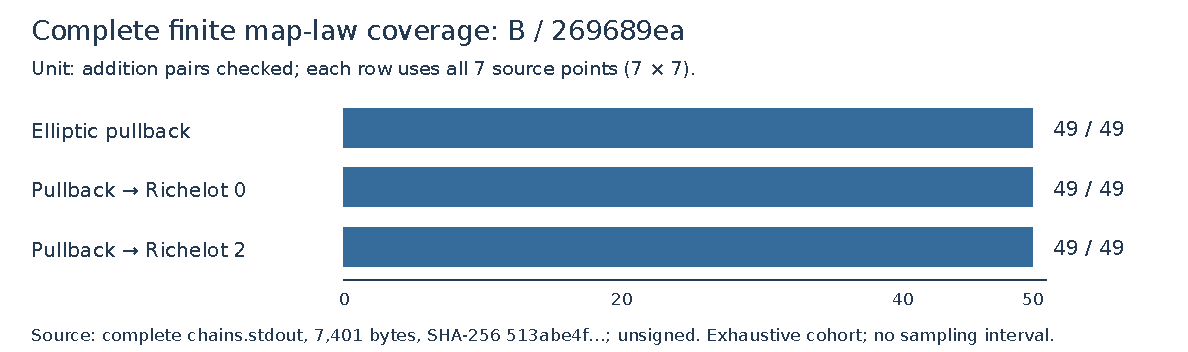
\includegraphics[width=0.98\linewidth]{coverage.pdf}\end{center}
\vspace{-3mm}
\textbf{Complete native output.} Source \texttt{269689ea}, result
\texttt{0aa75e14}, prospective record \texttt{1cce26}, data record
\texttt{35dbcf}. All $21$ image divisors, identity, order, Frobenius and
map-law checks are in \path{elliptic_chain/first-B-native/chains.stdout}:
$7{,}401$ bytes, SHA-256 prefix \texttt{513abe4f}. Transfer functions
consume only the public point and geometric coefficients; reference
scalar labels appear only in the control driver. \uv

\textbf{Scope.} This complete order-$7$ cohort qualifies these explicit
maps. A second map accepting arbitrary rational Jacobian classes, actual
Weil-$8$ pairing and cold comparative solver costs are separate next units.
No performance measurement was made in this qualification. \uv

\newpage
{\Large\bfseries Coordinates, exceptional points and controls}\par

\section{Working coordinates and reference checks}
The native field is $\mathbb F_{729}=\mathbb F_{27}[b]/(b^2-2)$ with
$\mathbb F_{27}=\mathbb F_3[a]/(a^3-a-1)$ and primitive element encoding
$30$. All $531{,}441$ pairs of addition and multiplication agree with
independent tower/trit formulas. All $729$ inverse, Frobenius-period and
square-root decisions pass, alongside basis distributivity controls.
The source elliptic law checks all $49$ additions and $343$ associativity
triples; invalid and noncanonical point controls are rejected. \uv

The written coordinate formulas use $u=x/(x+1)$ and $v=y/(x+1)^3$, then
$X=2u^2$, $Y=2v$. In a branch-root chart
$t=1/(x-r)$, $Z=yt^3/s$, the pullback is
\[
 u_D=\operatorname{monic}\big((rt+1)^2-2X((r+1)t+1)^2\big),\qquad
 v_D=(2Y/s)((r+1)t+1)^3\bmod u_D.
\]
Its two independently evaluated geometric preimages agree for every source
point, including a double preimage at $u=0$. The elliptic identity fibre is
a hyperelliptic conjugate pair and cancels. \uv

For source homogeneous coordinates $(a:b:y)$, the Richelot relation and
full ordinate numerator are
\[
 A(z)=G_0^h(a,b)H_0(z)+G_1^h(a,b)H_1(z),\quad
 N(z)=G_0^h(a,b)H_0(z)(a-bz)/y.
\]
At target branch root $w$, weights $2,3$ give
$\operatorname{monic}(t^2A(w+1/t))$ and
$t^3N(w+1/t)/s_{\rm target}$ reduced modulo the first polynomial.
The native tests use the full cubic numerator, including when $A$ is linear.
These formulas are readable derivations and native coefficient checks;
the formal/certificate gaps below remain explicit. \uv

\begin{center}\begin{tabular}{@{}L{0.37\linewidth}L{0.57\linewidth}@{}}
\toprule
Actual case or mutation & Native outcome and restoration\\\midrule
Original source infinities & Two preimages with $b=0$ are processed.\\
Omitted pullback scale $1/s$ & All six nonidentity images fail Mumford validity.\\
Moving branch-root Frobenius & All three charts reject omitted basepoint correction.\\
Degree drop: $x=20,25$, $y=1,2$ & All four full images valid; early affine reduction fails.\\
Regular counterpart: $x=0,y=1$ & Early reduction remains valid and gives the same class.\\
Product kernel, determinant $0$ & Smooth-Jacobian caller rejects the actual endpoint.\\
Nonidentity source points & All images nonzero, killed by $7$, distinct and $\mathbb F_3$-fixed.\\
\bottomrule\end{tabular}\end{center}

\section{Proof map and independent-validation scope}
Existing native Cantor function bodies are reused unchanged; independent
formulas check field operations and pullback fibres. The control driver is
same-author validation, not an external signed replay. Generic group laws,
the actual curve-to-Jacobian homomorphism bridge and axiom audit remain
open in \texttt{crypto-lean\#34}: local Mathlib imports failed and CI jobs
never started because of account billing lock. \uv

The existing \texttt{identity.certificate/v1} format fixes modulus
$2^{61}-1$. It cannot certify the characteristic-$3$ formulas as stated.
No such certificate or Lean theorem is asserted here; an integer-lift or
appropriate generic formal bridge must be separately checked. \uv

\newpage
{\Large\bfseries Genuine-curve evidence and preserved negatives}\par

\section{Earlier completed finite units in this lane}
\begin{center}\begin{tabular}{@{}L{0.30\linewidth}L{0.39\linewidth}L{0.22\linewidth}@{}}
\toprule
Unit and source & Actual complete native coverage & Raw / unsigned record\\\midrule
$\mathbb F_3$ census, \texttt{c37b4dfb} & $28$ cubic pairs, $48$ quintics;
$76$ smooth genus-$2$ curves; $1{,}296$ order checks & $28{,}832$ B;
\texttt{0700a8a4}; \texttt{0b48fa}\\
Actual $J[8]$, \texttt{0eac0c32} & $4{,}096$ canonical classes;
$16{,}384$ generator edges; actual Frobenius & $2{,}753$ B;
\texttt{d68b2673}; \texttt{5bd9de}\\
Richelot models, \texttt{0b292644} & $3$ stable kernels: $1$ product,
$2$ smooth; $52$ point ideals, $4$ degree drops & $6{,}283$ B;
\texttt{3599c111}; \texttt{c656d1}\\
Actual chains, \texttt{269689ea} & $3$ maps, $7$ points each;
$147$ additions, all exceptional controls & $7{,}401$ B;
\texttt{513abe4f}; \texttt{35dbcf}\\
\bottomrule\end{tabular}\end{center}
All rows are recorded native observations and remain unsigned. No unchanged
population was rerun for this report. \uv

For the selected actual curve, four order-$8$ divisor classes generate all
$4{,}096$ elements of $J[8]$ over $\mathbb F_{3^{12}}$. Actual coordinate
Frobenius on that basis and the separately evaluated two-torsion Weil form are
\[
 F_8=\begin{pmatrix}5&3&3&5\\2&4&6&3\\5&7&4&2\\4&5&0&1\end{pmatrix},\qquad
 e_2=\begin{pmatrix}0&0&1&0\\0&0&1&1\\1&1&0&0\\0&1&0&0\end{pmatrix}.
\]
The pairing matrix is $e_2$, not $e_8$. Fixed-class counts at Frobenius
powers $1,3,6,12$ are $1,16,256,4{,}096$; every image agrees with direct
coordinate Frobenius and all generator edges. \uv

\section{Negative results determine the next hypotheses}
In the fixed $3+3$ census, $16$ curves have split elliptic Weil factors and
horizon-$12$ two-adic valuation $12$. The other $12$ ordinary nonsplit curves
have valuation $16$: the preregistered nonsplit minimal-Sylow fixture is
absent from this finite family. This does not exclude other fields. \uv

All $48$ curves with branch type $5+1$ lack an elliptic Weil factor and have
horizon-$20$ valuation $12$. The written same-field argument uses irreducible
degree-$4$ Frobenius modulo $2$: the characteristic-zero Tate polynomial
cannot have a two-dimensional invariant elliptic factor. Its application
is to algebraic group morphisms over that field; broader computational
reductions and extension fields remain separate. Formalization is open. \uv

The old genus-$3$ finite kernel/RREF result is retained in parent PR5005,
but its endpoints are decomposable PPAVs. It supplies no smooth genus-$3$
Jacobian source. The written prospective successor is a fixed bielliptic
plane-quartic family over $\mathbb F_5$, with source and polarization gates
still unexecuted. \uv

\newpage
{\Large\bfseries Reproduction, first failures and continuation}\par

\section{Execution and first-failure flow}
Native Rust \texttt{1.99.1}, Linux x86-64 workspace; one worker,
$2$ GiB virtual address space and $120$ seconds per phase.
This earned bounded development/unit qualification, without isolated
benchmark admission or a timed comparison. Every successful source was
published and its entire frozen input closure read back before first phases.
Sources were separately copied, immutable qualifiers hashed before calls,
and build/pre-call/post-call guards retained. \uv

\begin{center}\begin{tabular}{@{}L{0.27\linewidth}L{0.65\linewidth}@{}}
\toprule
Fixed unit & Planned, attempted and retained outcomes\\\midrule
Census & A: formatting $1$; B: all seven phases $0$.\\
Actual coordinates & A: formatting $1$; B: unused import compile $1$;
C: inherited type-complexity Clippy $1$; D: all phases $0$.\\
Richelot codomains & A: formatting $1$; B: all seven phases $0$.\\
Explicit chains & A: formatting $1$, full $25{,}546$ B diagnostic;
B: all seven phases $0$, all source/tool/ELF guards unchanged.\\
Excluded by fixed rule & No old-population replay, paid job, original EKS-only
solver substitution or locked-vault execution.\\
\bottomrule\end{tabular}\end{center}
Each failure stops that profile; versioned repairs preserve its source and
complete diagnostics. No timeout, omitted target or failed arm is treated
as a success. Complete raw phase packets and result JSONs sit beside each
unit. Whole compiled ELFs and the $185{,}920$ B J8 coordinate table remain
in original private RAM custody pending a remote store or CI artifact;
these paths are temporary, not durable publication. \uv

\section{Requirements and next discriminating work}
\begin{center}\begin{tabular}{@{}L{0.33\linewidth}L{0.59\linewidth}@{}}
\toprule
Requested direction & Exact current state / next technical check\\\midrule
Nontrivial DLP-preserving maps & Explicit odd-order elliptic pullback and two
degree-$4$ Richelot maps qualified on the full order-$7$ cohort.\\
Chained Jacobian maps & Next: consume actual rational divisors at the second
hop; classify dual/backtracking and verify the exact raw $-[2]$ sign in char $3$.\\
Prime-field descent & All present map images pass corrected original
$\mathbb F_3$ Frobenius; rational model alone was not used as the test.\\
Computational advantage & Costs unmeasured. Freeze cold field/kernel/chart,
map, destination solve and scalar-replay accounting with the strongest
matched direct elliptic reference before calls.\\
Mathematical proof & Written derivations and native finite checks retained;
generic Mathlib/geometry/certificate bridges held, not waived.\\
Persistent queue / merge & Issue3904, local queue/RESUME and dated journal;
stacked draft5007 extends parent5005. Required CI failures remain held.\\
\bottomrule\end{tabular}\end{center}

\section{Sources and graph review}
\begin{flushleft}
Prior native sources: \path{src/cryptanalysis/jv_cover.rs}, blob
\texttt{990760b1}; and\\
\path{cd_attack/src/richelot.rs}, blob\texttt{2495980b}; existing cover/bielliptic implementations. Primary context:
Smith, \href{https://arxiv.org/abs/0806.2995}{arXiv:0806.2995v2}, especially
genus-$3$ descent/Serre obstruction; Bruin--Doerksen,
\href{https://arxiv.org/abs/0902.3480}{arXiv:0902.3480v3}; Magma Richelot
handbook, text1615. KB and Conductor unavailable; exact-source fallback is
not novelty clearance. \uv
\end{flushleft}

Canonical scoreboard, progress timeline, curve-transfer catalogs and
performance-gain figures were reviewed for scope. They remain unchanged:
this unsigned finite qualification has no admitted speed or leaderboard
row. The study graph and all rendered forms describe the exact new maps.
Full source-linked Markdown report, raw paths and build script accompany
this PDF. \uv

\href{https://github.com/isogeny-labs/crypto/pull/5007}{PR5007}\quad
\href{https://github.com/isogeny-labs/crypto/issues/3904}{Persistent queue3904}
\end{document}
